%
% File Name:	pgm_overview_2.tex
% Author:	Aditya Ramesh
% Date:		07/02/2012
% Contact:	cheesear@gmail.com
%

\documentclass[11pt]{beamer}
\usepackage[noend]{algorithmic}
\usepackage{amsfonts}
\usepackage{amsmath}
\usepackage{amssymb}
\usepackage{booktabs}
\usepackage{bbm}
\usepackage{breqn}
\usepackage{cancel}
\usepackage{caption}
\usepackage{colortbl}
\usepackage{graphicx}
\usepackage{multirow}
\usepackage{setspace}
\usepackage{subfig}
\usepackage{tikz}
\usepackage{url}
\usepackage{xfrac}
\usetikzlibrary{calc}
\usetikzlibrary{shapes.callouts}
\usetikzlibrary{shapes.multipart}
\usetheme{Singapore}
\usecolortheme{dove}

\captionsetup[subfigure]{position=top,labelformat=empty}
\title[PGM Overview]{%
	Overview of Probabilistic Graphical Models\\
	Representation: Part II
}
\author[Aditya Ramesh]{%
	Aditya Ramesh \\
	\footnotesize\texttt{\_@adityaramesh.com}
}
\institute[University of Delaware]{%
	John Cavazos Lab\\
	University of Delaware\\
	Newark, Delaware 19716
}
\date{}
\setbeamertemplate{itemize items}{\textbullet}

\tikzset{
	darkstyle/.style={circle,draw=black,fill=white!80!black},
	lightstyle/.style={circle,draw=black,fill=white},
	tablestyle/.style={rectangle,fill=white},
	factorstyle/.style={rectangle,draw=black,fill=white!80!black}
}

\begin{document}

\begin{frame}[plain]
\titlepage
\footnotesize
This presentation is based \textbf{heavily} on the material by Daphne Koller
(\cite{pgmbook}), Nir Friedman (\cite{pgmbook}, \cite{nirslides}), and David
Sontag (\cite{pgmslides}). I have \textbf{directly copied} or otherwise
incorporated parts of their work into many of these slides, citing the sources
where appropriate. If you find this presentation useful, I highly recommend that
you take some time to read their work.
\end{frame}

\begin{frame}
\frametitle{Outline}
\tableofcontents
\end{frame}

\section{Conversion between Networks \cite{pgmbook}}
\subsection{Motivation}

\begin{frame}{Motivation}
\begin{itemize}
	\item We saw earlier with the Misconception example that we cannot
	easily express interactions between cliques in Bayesian networks.
	\item Recall the conditions under which the common effect v-structure
	in Bayesian networks ($X \rightarrow Y \leftarrow Z$) is active.
	\item We cannot represent these types of independencies in Markov
	networks.
\end{itemize}
\end{frame}

\begin{frame}{Motivation}
\begin{itemize}
	\item Each type of network can represent independence constraints that
	the other cannot.
	\item A natural question to ask is the following: when can we convert
	one type of network to another?
	\item We will first develop a procedure to convert a Bayesian network to
	a Markov network, and find the conditions under which the transformation
	is ``lossless''.
\end{itemize}
\end{frame}

\subsection{Bayesian Networks to Markov Networks}

\begin{frame}{Bayesian Networks to Markov Networks}
\begin{itemize}
	\item We define the \emph{reduction} of the factor $\phi$ to the context
	$\boldsymbol{U} = \boldsymbol{u}$, denoted $\phi[\boldsymbol{U} =
	\boldsymbol{u}]$ (and abbreviated $\phi[\boldsymbol{u}]$), to be a
	factor over scope $\boldsymbol{Y}' = \boldsymbol{Y} - \boldsymbol{U}$,
	such that
	\[
		\phi[\boldsymbol{u}](\boldsymbol{y}') = \phi(\boldsymbol{y}',
		\boldsymbol{u}).
	\]
	\item A Bayesian network conditioned on evidence $\boldsymbol{E} =
	\boldsymbol{e}$ also induces a Gibbs distribution: the one defined by
	the original factors \emph{reduced} to the context $\boldsymbol{E} =
	\boldsymbol{e}$.
\end{itemize}
\end{frame}

\begin{frame}{Bayesian Networks to Markov Networks}
\begin{itemize}
	\item A Markov network has the restriction that all variables belonging
	to the scope of a factor must be in the same clique.
	\item If we want to come up with a procedure to convert a Bayesian
	network to an undirected representation, we have to find some way of
	dealing with v-structures of the form $X \rightarrow Z \leftarrow Y$.
	\item Solution: \emph{moralize} the network by ``marrying'' unconnected
	parents of the same node.
\end{itemize}
\end{frame}

\begin{frame}{Bayesian Networks to Markov Networks}
\begin{itemize}
	\item The moralized graph $\mathcal{M}[G]$ is clearly an I-map for
	any distribution $P$ parameterized over $G$.
	\item However, it is only a perfect map when we did not have any
	\emph{immoralities} in the Bayesian network to begin with.
	\item Otherwise, we have lost independence information through the
	addition of moralizing edges.
	\item Caveat: we rarely encounter a directed graph that is moral. The
	transformation is likely to be ``lossy''.
\end{itemize}
\end{frame}

\subsection{Markov Networks to Bayesian Networks}

\captionsetup[subfigure]{position=bottom,labelformat=empty}

\newcommand{\markovtobayesian}
{
	\subfloat[][(a)]
	{%
		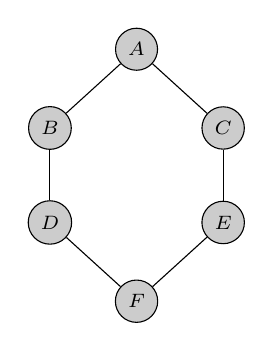
\begin{tikzpicture}
		\scriptsize
		\node[darkstyle] (a) at (0,1.6) {$A$};
		\node[darkstyle] (b) at (-1.1,0.6) {$B$};
		\node[darkstyle] (c) at (1.1,0.6) {$C$};
		\node[darkstyle] (d) at (-1.1,-0.6) {$D$};
		\node[darkstyle] (e) at (1.1,-0.6) {$E$};
		\node[darkstyle] (f) at (0,-1.6) {$F$};
		\draw (a)--(b);
		\draw (a)--(c);
		\draw (b)--(d);
		\draw (c)--(e);
		\draw (d)--(f);
		\draw (e)--(f);
		\end{tikzpicture}
	}%
	\hspace{1.0cm}
	\subfloat[][(b)]
	{%
		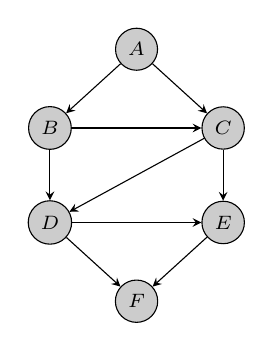
\begin{tikzpicture}
		\scriptsize
		\node[darkstyle] (a) at (0,1.6) {$A$};
		\node[darkstyle] (b) at (-1.1,0.6) {$B$};
		\node[darkstyle] (c) at (1.1,0.6) {$C$};
		\node[darkstyle] (d) at (-1.1,-0.6) {$D$};
		\node[darkstyle] (e) at (1.1,-0.6) {$E$};
		\node[darkstyle] (f) at (0,-1.6) {$F$};
		\draw[-stealth] (a)--(b);
		\draw[-stealth] (a)--(c);
		\draw[-stealth] (b)--(d);
		\draw[-stealth] (c)--(e);
		\draw[-stealth] (d)--(f);
		\draw[-stealth] (e)--(f);
		\draw[-stealth] (b)--(c);
		\draw[-stealth] (c)--(d);
		\draw[-stealth] (d)--(e);
		\end{tikzpicture}
	}
}

\begin{frame}{Markov Networks to Bayesian Networks}
\setlength{\topsep}{0pt}
\setlength{\partopsep}{0pt}
\centering
\begin{figure}
\resizebox{0.6\textwidth}{!}{\markovtobayesian}
\end{figure}
\begin{itemize}
	\item The procedure to transform a Markov network into a Bayesian
	network is more subtle, so we will first focus on an example.
	\item We aim to find a Bayesian network $G$ that is a minimal I-map for
	the Markov network $H$ shown in (a).
	\item Enumerating the nodes of $H$ in the order $A,B,C,D,E,F$, and
	ensuring that the independencies $I(H)$ are satisfied, results in the
	Bayesian network minimal I-map shown in (b).
\end{itemize}
\end{frame}

\begin{frame}{Markov Networks to Bayesian Networks}
\setlength{\topsep}{0pt}
\setlength{\partopsep}{0pt}
\centering
\begin{figure}
\resizebox{0.6\textwidth}{!}{\markovtobayesian}
\end{figure}
\begin{itemize}
	\item It turns out that any Bayesian network minimal I-map for an
	undirected graph $H$ can have no immoralities, and is necessarily
	chordal (the longest loop is of length 3).
	\item The process of adding enough edges to a Markov network to turn it
	into a Bayesian network is called \emph{triangulation}.
\end{itemize}
\end{frame}

\begin{frame}{Markov Networks to Bayesian Networks}
\begin{itemize}
	\item The ordering of nodes we determined for the previous example can
	be thought of as derived from the ordering of cliques in the
	\emph{clique tree} embedded in the undirected graph.
	\item In the previous example, each clique in the tree consists of
	exactly one node.
	\item When we generalize this approach to cliques containing many nodes,
	we need to formalize what it means for two cliques to be ``separated''.
\end{itemize}
\end{frame}

\begin{frame}{Markov Networks to Bayesian Networks}
\begin{itemize}
	\item Let $\boldsymbol{C}_{i},\boldsymbol{C}_{j}$ be two (necessarily
	maximal) cliques in a clique tree that are directly connected by an
	edge.
	\begin{itemize}
		\item We define $\boldsymbol{S}_{i,j} = \boldsymbol{C}_{i} \cap
		\boldsymbol{C}_{j}$ to be the \emph{sepset} between
		$\boldsymbol{C}_{i}$ and $\boldsymbol{C}_{j}$.
		\item The sepset $\boldsymbol{S}_{i,j}$ is the minimal set of
		nodes that need to be observed to render $\boldsymbol{C}_{i}$
		and $\boldsymbol{C}_{j}$ conditionally independent.
		\item Let $\boldsymbol{W}_{<(i,j)}$ ($\boldsymbol{W}_{<(j,i)}$)
		be all of the variables that appear in any clique on the
		$\boldsymbol{C}_{i}$ ($\boldsymbol{C}_{j}$) side of the edge.
		\item Each edge decomposes $\mathcal{X}$ into three disjoint
		sets: $\boldsymbol{W}_{<(i,j)} - \boldsymbol{S}_{i,j}$,
		$\boldsymbol{W}_{<(j,i)} - \boldsymbol{S}_{i,j}$, and
		$\boldsymbol{S}_{i,j}$.
	\end{itemize}
\end{itemize}
\end{frame}

\begin{frame}{Markov Networks to Bayesian Networks}
\begin{itemize}
	\item We say that a tree $T$ is a clique tree for $H$ if:
	\begin{itemize}
		\item each node corresponds to a clique in $H$, and each maximal
		clique in $H$ is a node in $T$;
		\item each sepset $\boldsymbol{S}_{i,j}$ separates
		$\boldsymbol{W}_{<(i,j)}$ and $\boldsymbol{W}_{<(j,i)}$ in $H$.
	\end{itemize}
	\item In other words, the clique tree describes the connections between
	the set of maximal cliques in $H$, such that observing the sepset
	between two cliques in the tree renders them conditionally independent.
\end{itemize}
\end{frame}

\begin{frame}{Markov Networks to Bayesian Networks}
\begin{itemize}
	\item To generalize our procedure to convert a given Markov network $H$
	to a Bayesian network $G$, we do the following:
	\begin{enumerate}
		\pause
		\item Select an arbitrary clique $\boldsymbol{C}_{1}$ to be the
		root of the clique tree.
		\pause
		\item Order the cliques $\boldsymbol{C}_{1}, \ldots,
		\boldsymbol{C}_{k}$ using any topological ordering such that the
		cliques closer to the root appear first.
		\pause
		\item Order the nodes in any order consistent with the clique
		ordering: if $X_{l}$ first appears in $\boldsymbol{C}_{i}$ and
		$X_{m}$ first appears in $\boldsymbol{C}_{j}$, for $i < j$, then
		$X_{l}$ must precede $X_{m}$ in the ordering.
		\pause
		\item Use the algorithm discussed in the first talk (repeated
		shortly) to build a minimal I-map given the ordering $X_{1},
		\ldots, X_{n}$ and independencies $I(H)$.
	\end{enumerate}
\end{itemize}
\end{frame}

\begin{frame}{Algorithm for Constructing a Minimal I-Map}
\setlength{\topsep}{0pt}
\setlength{\partopsep}{0pt}
\vspace{0pt}
\begin{algorithmic}
\REQUIRE An ordering $X_{1}, \ldots, X_{n}$ of random variables in $\mathcal{X}$
\REQUIRE A set of independencies $I$
\pause
\STATE Set $G$ to an empty graph over $\mathcal{X}$
\pause
\FOR{$i = 1, \ldots, n$}
	\STATE{\textcolor{gray}{$\boldsymbol{U}$ is the current candidate for
	parents of $X_{i}$}}
	\STATE $\boldsymbol{U} \leftarrow \{X_{1}, \ldots, X_{i-1}\}$
	\pause
	\STATE{\textcolor{gray}{Find the minimal set $\boldsymbol{U}$ satisfying
	$(X_{i} \perp \{X_{1}, \ldots, X_{i-1}\} - \boldsymbol{U} \;|\;
	\boldsymbol{U})$}}
	\FOR{$\boldsymbol{U'} \subseteq \{X_{1}, \ldots, X_{i-1}\}$}
		\IF{$\boldsymbol{U'} \subset \boldsymbol{U}$ and $(X_{i} \perp
		\{X_{1}, \ldots, X_{i-1}\} - \boldsymbol{U'} \;|\;
		\boldsymbol{U'}) \in I$}
			\STATE{$\boldsymbol{U} \leftarrow \boldsymbol{U'}$}
		\ENDIF
	\ENDFOR
	\pause
	\STATE{\textcolor{gray}{Now set $\boldsymbol{U}$ to be the parents of
	$X_{i}$}}
	\FOR{$X_{i} \in \boldsymbol{U}$}
		\STATE{Add $X_{j} \text{---} X_{i}$ to $G$}
	\ENDFOR
	\pause
	\RETURN{$G$}
\ENDFOR
\end{algorithmic}
\end{frame}

\begin{frame}{Markov Networks to Bayesian Networks}
\setlength{\topsep}{0pt}
\setlength{\partopsep}{0pt}
\vspace{0pt}
\centering
\begin{figure}[!t]
\resizebox{0.2\textwidth}{!}{%
	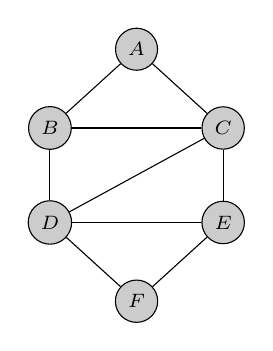
\begin{tikzpicture}
	\scriptsize
	\node[darkstyle] (a) at (0,1.6) {$A$};
	\node[darkstyle] (b) at (-1.1,0.6) {$B$};
	\node[darkstyle] (c) at (1.1,0.6) {$C$};
	\node[darkstyle] (d) at (-1.1,-0.6) {$D$};
	\node[darkstyle] (e) at (1.1,-0.6) {$E$};
	\node[darkstyle] (f) at (0,-1.6) {$F$};
	\draw (a)--(b);
	\draw (a)--(c);
	\draw (b)--(d);
	\draw (c)--(e);
	\draw (d)--(f);
	\draw (e)--(f);
	\draw (b)--(c);
	\draw (c)--(d);
	\draw (d)--(e);
	\end{tikzpicture}
}
\caption*{\centering\scriptsize The clique tree for the graph $H$ shown above is
a chain $\{A,B,C\} \rightarrow \{B,C,D\} \rightarrow \{C,D,E\} \rightarrow
\{D,E,F\}$.}
\end{figure}
\begin{itemize}
	\item It turns out that every undirected graph $H$ has a clique tree
	$T$.
	\item If $H$ is a nonchordal Markov network, then there is no Bayesian
	network $G$ that is a perfect map for $H$.
	\item On the other hand, if $H$ is a chordal Markov network, then there
	is a Bayesian network $G$ such that $I(H) = I(G)$, and it can be found
	using the procedure we just discussed.
\end{itemize}
\end{frame}

\section{Partially Directed Models \cite{pgmbook}}
\subsection{Motivation}

\begin{frame}{Motivation}
\begin{itemize}
	\item Consider a set of variables $\mathcal{X} = \boldsymbol{X} \cup
	\boldsymbol{Y}$, where $\boldsymbol{Y}$ is a set of \emph{target
	variables} and $\boldsymbol{X}$ is a (disjoint) set of \emph{observed
	variables}.
	\item The dependencies among the variables in $\boldsymbol{X}$ may be
	quite complex and poorly understood.
\end{itemize}
\end{frame}

\begin{frame}{Motivation}
\begin{itemize}
	\item So far, we have been trying to model the joint distribution
	$P(\boldsymbol{Y}, \boldsymbol{X})$; we could instead try modeling the
	distribution $P(\boldsymbol{Y} \;|\; \boldsymbol{X})$.
	\item By introducing directed dependencies between the $\boldsymbol{Y}$
	and $\boldsymbol{X}$, we can avoid encoding the distribution
	$P(\boldsymbol{X})$ altogether. In other words, we disallow any factor
	whose scope is a subset of $\boldsymbol{X}$.
	\item This allows us to focus on using our domain knowledge to encode a
	rich set of features into the model.
\end{itemize}
\end{frame}

\begin{frame}{Conditional Random Fields}
\begin{itemize}
	\item A \emph{conditional random field} is an undirected graph $H$ whose
	nodes correspond to $\boldsymbol{X} \cup \boldsymbol{Y}$; the network is
	annotated with a set of factors $\phi_{1}(\boldsymbol{D}_{1}), \ldots,
	\phi_{m}(\boldsymbol{D}_{m})$ \textcolor{blue}{such that each
	$\boldsymbol{D}_{i} \nsubseteq \boldsymbol{X}$.} The network encodes a
	distribution as follows:
	\begin{align*}
		P(\boldsymbol{Y} \;|\; \boldsymbol{X}) &=
		\frac{1}{\boldsymbol{Z}(\boldsymbol{X})}
		\tilde{P}(\boldsymbol{Y},\boldsymbol{X}) \\
		\tilde{P}(\boldsymbol{Y},\boldsymbol{X}) &=
		\prod_{i=1}^{m} \phi_{i}(\boldsymbol{D}_{i}) \\
		Z(\boldsymbol{X}) &= \sum_{\boldsymbol{Y}}
		\tilde{P}(\boldsymbol{Y}, \boldsymbol{X}).
	\end{align*}
\end{itemize}
\end{frame}

\subsection{Conditional Random Fields}

\newcommand{\linearchain}
{
	\subfloat[][(a)]
	{%
		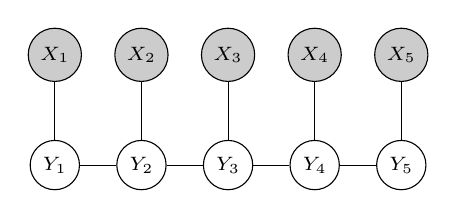
\begin{tikzpicture}
		\scriptsize
		\node[lightstyle] (y1) at (-2.2,0) {$Y_{1}$};
		\node[lightstyle] (y2) at (-1.1,0) {$Y_{2}$};
		\node[lightstyle] (y3) at (0,0) {$Y_{3}$};
		\node[lightstyle] (y4) at (1.1,0) {$Y_{4}$};
		\node[lightstyle] (y5) at (2.2,0) {$Y_{5}$};
		\node[darkstyle] (x1) at (-2.2,1.4) {$X_{1}$};
		\node[darkstyle] (x2) at (-1.1,1.4) {$X_{2}$};
		\node[darkstyle] (x3) at (0,1.4) {$X_{3}$};
		\node[darkstyle] (x4) at (1.1,1.4) {$X_{4}$};
		\node[darkstyle] (x5) at (2.2,1.4) {$X_{5}$};
		\draw (y1)--(y2);
		\draw (y2)--(y3);
		\draw (y3)--(y4);
		\draw (y4)--(y5);
		\draw (x1)--(y1);
		\draw (x2)--(y2);
		\draw (x3)--(y3);
		\draw (x4)--(y4);
		\draw (x5)--(y5);
		\end{tikzpicture}
	}%
	\hspace{0.5cm}
	\subfloat[][(b)]
	{%
		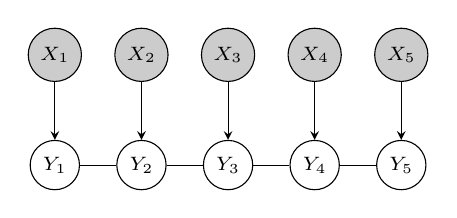
\begin{tikzpicture}
		\scriptsize
		\node[lightstyle] (y1) at (-2.2,0) {$Y_{1}$};
		\node[lightstyle] (y2) at (-1.1,0) {$Y_{2}$};
		\node[lightstyle] (y3) at (0,0) {$Y_{3}$};
		\node[lightstyle] (y4) at (1.1,0) {$Y_{4}$};
		\node[lightstyle] (y5) at (2.2,0) {$Y_{5}$};
		\node[darkstyle] (x1) at (-2.2,1.4) {$X_{1}$};
		\node[darkstyle] (x2) at (-1.1,1.4) {$X_{2}$};
		\node[darkstyle] (x3) at (0,1.4) {$X_{3}$};
		\node[darkstyle] (x4) at (1.1,1.4) {$X_{4}$};
		\node[darkstyle] (x5) at (2.2,1.4) {$X_{5}$};
		\draw (y1)--(y2);
		\draw (y2)--(y3);
		\draw (y3)--(y4);
		\draw (y4)--(y5);
		\draw[-stealth] (x1)--(y1);
		\draw[-stealth] (x2)--(y2);
		\draw[-stealth] (x3)--(y3);
		\draw[-stealth] (x4)--(y4);
		\draw[-stealth] (x5)--(y5);
		\end{tikzpicture}
	}%
	\hspace{0.5cm}
	\subfloat[][(c)]
	{%
		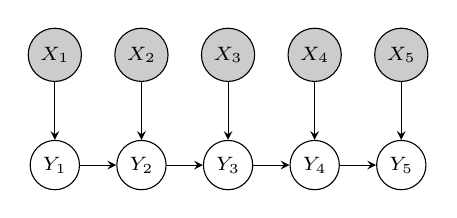
\begin{tikzpicture}
		\scriptsize
		\node[lightstyle] (y1) at (-2.2,0) {$Y_{1}$};
		\node[lightstyle] (y2) at (-1.1,0) {$Y_{2}$};
		\node[lightstyle] (y3) at (0,0) {$Y_{3}$};
		\node[lightstyle] (y4) at (1.1,0) {$Y_{4}$};
		\node[lightstyle] (y5) at (2.2,0) {$Y_{5}$};
		\node[darkstyle] (x1) at (-2.2,1.4) {$X_{1}$};
		\node[darkstyle] (x2) at (-1.1,1.4) {$X_{2}$};
		\node[darkstyle] (x3) at (0,1.4) {$X_{3}$};
		\node[darkstyle] (x4) at (1.1,1.4) {$X_{4}$};
		\node[darkstyle] (x5) at (2.2,1.4) {$X_{5}$};
		\draw[-stealth] (y1)--(y2);
		\draw[-stealth] (y2)--(y3);
		\draw[-stealth] (y3)--(y4);
		\draw[-stealth] (y4)--(y5);
		\draw[-stealth] (x1)--(y1);
		\draw[-stealth] (x2)--(y2);
		\draw[-stealth] (x3)--(y3);
		\draw[-stealth] (x4)--(y4);
		\draw[-stealth] (x5)--(y5);
		\end{tikzpicture}
	}
}

\begin{frame}{Conditional Random Fields}
\vspace{0.35cm}
\setlength{\topsep}{0pt}
\setlength{\partopsep}{0pt}
\begin{figure}[!t]
\resizebox{0.85\textwidth}{!}{\linearchain}
\end{figure}
\vspace{0.35cm}
\begin{itemize}
	\item The undirected CRF shown in (a) has the form:
	\begin{align*}
	P(\boldsymbol{Y} \;|\; \boldsymbol{X}) &= \frac{1}{Z(\boldsymbol{X})}
	\tilde{P}(\boldsymbol{Y},\boldsymbol{X}) \\
	\tilde{P}(\boldsymbol{Y},\boldsymbol{X}) &=
	\prod_{i=1}^{k-1} \phi(Y_{i},Y_{i+1}) \prod_{i=1}^{k} \phi(Y_{i},X_{i})
	\\
	Z(\boldsymbol{X}) &= \sum_{\boldsymbol{Y}} \tilde{P}(\boldsymbol{Y},
	\boldsymbol{X}).
	\end{align*}
	\item The partially directed CRF shown in (b) is equivalent.
\end{itemize}
\end{frame}

\begin{frame}{Conditional Random Fields}
\vspace{0.35cm}
\setlength{\topsep}{0pt}
\setlength{\partopsep}{0pt}
\begin{figure}[!t]
\resizebox{0.85\textwidth}{!}{\linearchain}
\end{figure}
\vspace{0.35cm}
\begin{itemize}
	\item The Bayesian network in (c) is not equivalent to (a) or (b), as it
	implies that $(Y_{i} \perp X_{i+1})$ (recall the common effect
	v-structure $X \rightarrow Z \leftarrow Y$).
	\item In the CRFs shown in (a) and (b), the unnormalized measure of
	$\boldsymbol{Y}$ depends on the entire parameterization of the chain
	(the assignment to $\boldsymbol{X}$).
	\item To encode these dependencies in (c), we would have to draw edges
	from all the variables in $\boldsymbol{X}$ to each of the variables in
	$\boldsymbol{Y}$.
\end{itemize}
\end{frame}

\begin{frame}{Conditional Random Fields}
\begin{itemize}
	\item Factors in conditional random fields are typically parameterized
	as log-linear functions, which were discussed in the first talk.
	\item Consider a CRF over the binary-valued variables $\boldsymbol{X} =
	\{ X_{1}, \ldots, X_{k} \}$ and $Y$, and a pairwise potential between
	each $Y$ and each $X_{i}$ (aka the \emph{naive Markov model}).
	\item We parameterize the potentials as follows:
	\begin{align*}
		\phi_{i}(X_{i},Y) &= \text{exp}\{w_{i}\mathbbm{1}
		\{X_{i} = 1, Y = 1\}\} \\
		\phi_{0}(Y) &= \text{exp}\{w_{0}\mathbbm{1}\{Y=1\}\}.
	\end{align*}
\end{itemize}
\end{frame}

\begin{frame}{Conditional Random Fields}
\begin{itemize}
	\item We have
	\begin{align*}
		\tilde{P}(Y = 1 \;|\; x_{1}, \ldots, x_{k}) &= \text{exp}\left\{
		w_{0} + \sum_{i=1}^{k} w_{i}x_{i}\right\}\\
		\tilde{P}(Y = 0 \;|\; x_{1}, \ldots, x_{k}) &= \text{exp}(0) =
		1,
	\end{align*}
	so
	\begin{align*}
		P(Y = 1 \;|\; x_{1}, &\ldots, x_{k})\\ &= \frac{1}{Z(x_{1}, \ldots,
		x_{k})} \tilde{P}(Y = 1 \;|\; x_{1}, \ldots, x_{k})\\
		&= \frac{\tilde{P}(Y = 1 \;|\; x_{1}, \ldots, x_{k})}
		{\tilde{P}(Y = 0 \;|\; x_{1}, \ldots, x_{k}) +
		\tilde{P}(Y = 1 \;|\; x_{1}, \ldots, x_{k})}\\
		&= \text{sigmoid}\left(w_{0} + \sum_{i=1}^{k} w_{i}x_{i}\right).
	\end{align*}
\end{itemize}
\end{frame}

\subsection{Named-Entity Recognition}

\begin{frame}{Named-Entity Recognition \cite{pgmslides}}
\begin{itemize}
	\item Given a sentence, determine the people and organizations involved,
	along with their relevant locations in the sentence: ``Mrs. Green spoke
	today in New York. Green chairs the finance committee.''
	\item Entities sometimes span multiple words. The entity of a word is
	not obvious without considering its \emph{context}.
\end{itemize}
\end{frame}

\begin{frame}{Named-Entity Recognition \cite{pgmslides}}
\begin{itemize}
	\item The CRF has one variable $X_{i}$ for each word, which encodes the
	possible labels of that word.
	\item The targets are, for example, ``B-person'', ``I-person'',
	``B-location'', ``I-location'', ``B-organization'', and
	``I-organization''.
	\item Having ``B'' mark the beginning of an entity and ``I'' mark the
	inside or end of an entity allows the model to segment adjacent
	entities.
\end{itemize}
\end{frame}

\newcommand{\nerexample}
{%
	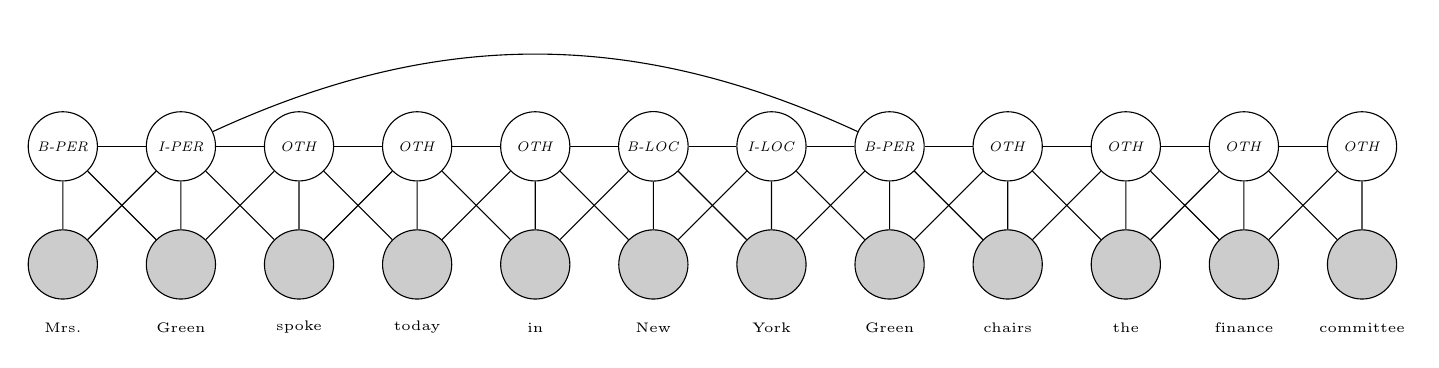
\begin{tikzpicture}
	\tiny
	\node[lightstyle,minimum size=25] (a) at (-8.25,0) {\textit{B-PER}};
	\node[lightstyle,minimum size=25] (b) at (-6.75,0) {\textit{I-PER}};
	\node[lightstyle,minimum size=25] (c) at (-5.25,0) {\textit{OTH}};
	\node[lightstyle,minimum size=25] (d) at (-3.75,0) {\textit{OTH}};
	\node[lightstyle,minimum size=25] (e) at (-2.25,0) {\textit{OTH}};
	\node[lightstyle,minimum size=25] (f) at (-0.75,0) {\textit{B-LOC}};
	\node[lightstyle,minimum size=25] (g) at (0.75,0) {\textit{I-LOC}};
	\node[lightstyle,minimum size=25] (h) at (2.25,0) {\textit{B-PER}};
	\node[lightstyle,minimum size=25] (i) at (3.75,0) {\textit{OTH}};
	\node[lightstyle,minimum size=25] (j) at (5.25,0) {\textit{OTH}};
	\node[lightstyle,minimum size=25] (k) at (6.75,0) {\textit{OTH}};
	\node[lightstyle,minimum size=25] (l) at (8.25,0) {\textit{OTH}};
	\node[darkstyle,minimum size=25] (aa) at (-8.25,-1.5) {};
	\node[darkstyle,minimum size=25] (bb) at (-6.75,-1.5) {};
	\node[darkstyle,minimum size=25] (cc) at (-5.25,-1.5) {};
	\node[darkstyle,minimum size=25] (dd) at (-3.75,-1.5) {};
	\node[darkstyle,minimum size=25] (ee) at (-2.25,-1.5) {};
	\node[darkstyle,minimum size=25] (ff) at (-0.75,-1.5) {};
	\node[darkstyle,minimum size=25] (gg) at (0.75,-1.5) {};
	\node[darkstyle,minimum size=25] (hh) at (2.25,-1.5) {};
	\node[darkstyle,minimum size=25] (ii) at (3.75,-1.5) {};
	\node[darkstyle,minimum size=25] (jj) at (5.25,-1.5) {};
	\node[darkstyle,minimum size=25] (kk) at (6.75,-1.5) {};
	\node[darkstyle,minimum size=25] (ll) at (8.25,-1.5) {};
	\draw (a)--(b) (b)--(c) (c)--(d) (d)--(e) (e)--(f) (f)--(g) (g)--(h)
	(h)--(i) (i)--(j) (j)--(k) (k)--(l);
	\draw (b) .. controls (-3.5,1.5) and (-1.0,1.5) .. (h);
	\draw (a)--(aa) (a)--(bb);
	\draw (b)--(aa) (b)--(bb) (b)--(cc);
	\draw (c)--(bb) (c)--(cc) (c)--(dd);
	\draw (d)--(cc) (d)--(dd) (d)--(ee);
	\draw (e)--(dd) (e)--(ee) (e)--(ff);
	\draw (f)--(ee) (f)--(ff) (f)--(gg);
	\draw (g)--(ff) (g)--(gg) (g)--(hh);
	\draw (h)--(gg) (h)--(hh) (h)--(ii);
	\draw (i)--(hh) (i)--(ii) (i)--(jj);
	\draw (j)--(ii) (j)--(jj) (j)--(kk);
	\draw (k)--(jj) (k)--(kk) (k)--(ll);
	\draw (l)--(kk) (l)--(ll);
	\node (at) at (-8.25,-2.3) {Mrs.};
	\node (bt) at (-6.75,-2.3) {Green};
	\node (ct) at (-5.25,-2.3) {spoke};
	\node (dt) at (-3.75,-2.3) {today};
	\node (et) at (-2.25,-2.3) {in};
	\node (ft) at (-0.75,-2.3) {New};
	\node (gt) at (0.75,-2.3) {York};
	\node (ht) at (2.25,-2.3) {Green};
	\node (it) at (3.75,-2.3) {chairs};
	\node (jt) at (5.25,-2.3) {the};
	\node (kt) at (6.75,-2.3) {finance};
	\node (lt) at (8.25,-2.3) {committee};
	\end{tikzpicture}
}

\begin{frame}{NLP Example: Named-Entity Recognition \cite{pgmslides}}
\setlength{\topsep}{0pt}
\setlength{\partopsep}{0pt}
\centering
\resizebox{0.8\textwidth}{!}{\nerexample}
\begin{itemize}
	\item This is typically represented by having two factors for each word:
	\begin{itemize}
		\item $\phi^{1}(Y_{t},Y_{t+1})$ represents the dependencies
		between neighboring target variables.
		\item $\phi^{2}(Y_{t},X_{1},\ldots,X_{T})$ represents the
		dependencies between a target and its context in the word
		sequence.
	\end{itemize}
\end{itemize}
\end{frame}

\begin{frame}{NLP Example: Named-Entity Recognition \cite{pgmslides}}
\setlength{\topsep}{0pt}
\setlength{\partopsep}{0pt}
\centering
\resizebox{0.8\textwidth}{!}{\nerexample}
\begin{itemize}
	\item A large number of features of the word $X_{t}$ and its neighboring
	words are relevant to the named entity decision (e.g. whether it is
	capitalized, appears in a list of common person names, appears in an
	atlas of common names, ends in the string ``ton'', or is exactly the
	string ``York'' followed by the word ``Times'').
\end{itemize}
\end{frame}

\begin{frame}{NLP Example: Named-Entity Recognition \cite{pgmslides}}
\setlength{\topsep}{0pt}
\setlength{\partopsep}{0pt}
\centering
\resizebox{0.8\textwidth}{!}{\nerexample}
\begin{itemize}
	\item These features are often sparse, though highly indicative.
	\item A common practice is to connect identical words together, in order
	to enforce that they are assigned to the same labels.
	\item Such a CRF is called a linear-chain CRF, and achieves accuracies
	in the high 90 percent range on many natural data sets.
\end{itemize}
\end{frame}

\subsection{Chain Graphs}

\begin{frame}{Chain Graphs}
\begin{itemize}
	\item We can generalize our ideas used to formulate the notion of the
	conditional random field by allowing arbitrary, undirected \emph{chain
	components} in a PDAG to be connected to one another in a directed
	fashion.
	\item We will begin by formalizing the notion of the chain component,
	and thus the notion of the chain graph.
\end{itemize}
\end{frame}

\begin{frame}{Chain Graphs}
\begin{itemize}
	\item Let $K$ be a PDAG over $\mathcal{X}$. Let $\boldsymbol{K}_{1},
	\ldots, \boldsymbol{K}_{l}$ be a disjoint partition of $\mathcal{X}$
	such that:
	\begin{itemize}
		\item the induced subgraph over $\boldsymbol{K}_{i}$ contains no
		directed edges;
		\item for any pair of nodes $X \in \boldsymbol{K}_{i}$ and $Y
		\in \boldsymbol{K}_{j}$ for $i < j$, an edge between $X$ and $Y$
		can only be a directed edge $X \rightarrow Y$.
	\end{itemize}
	\item Each component $\boldsymbol{K}_{i}$ is called a chain componment.
	\item Because of its chain structure, a PDAG is also called a
	\emph{chain graph}.
\end{itemize}
\end{frame}

\begin{frame}{Chain Graphs}
\begin{itemize}
	\item In a PDAG, we have both the notion of parents of $X$ (variables
	$Y$ such that $Y \rightarrow X$) and neighbors of $X$ (variables $Y$
	such that $Y \text{---} X$).
	\item The union of these two sets is the \emph{boundary} of $X$, denoted
	$\text{Boundary}_{X}$.
\end{itemize}
\end{frame}

\begin{frame}{Chain Graphs}
\begin{itemize}
	\item We say that a subset of nodes $\boldsymbol{X} \in \mathcal{X}$ is
	\emph{upwardly closed} in $K$ if, \textcolor{blue}{for any $X \in
	\boldsymbol{X}$, we have that $\text{Boundary}_{X} \subset
	\boldsymbol{X}$}.
	\item We define the \emph{upward closure} of $\boldsymbol{X}$ to be the
	minimal upwardly closed subset $\boldsymbol{Y}$ that contains
	$\boldsymbol{X}$.
	\item The definition of the upward closure of $X$ is somewhat subtle.
	Obviously the upward closure $\boldsymbol{Y}$ must contain
	$\boldsymbol{X}$. But this means that for all $U \in
	\text{Boundary}_{\boldsymbol{X}}$, we must also have $U \in
	\boldsymbol{Y}$.
	\item So to obtain the upward closure $\boldsymbol{Y}$ of
	$\boldsymbol{X}$, we must recursively add the boundaries of all nodes in
	$\boldsymbol{Y}$ until we cannot proceed any further.
\end{itemize}
\end{frame}

\newcommand{\upwardclosure}
{%
	\subfloat[][(a)]
	{%
		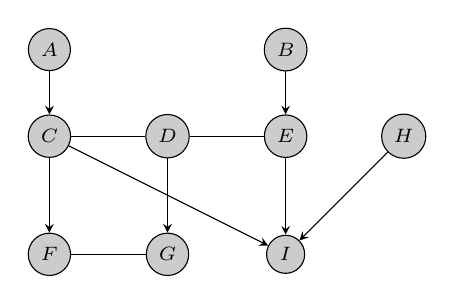
\begin{tikzpicture}
		\scriptsize
		\node[darkstyle] (a) at (-1.5,1.1) {$A$};
		\node[darkstyle] (c) at (-1.5,0) {$C$};
		\node[darkstyle] (d) at (0,0) {$D$};
		\node[darkstyle] (e) at (1.5,0) {$E$};
		\node[darkstyle] (b) at (1.5,1.1) {$B$};
		\node[darkstyle] (f) at (-1.5,-1.5) {$F$};
		\node[darkstyle] (g) at (0,-1.5) {$G$};
		\node[darkstyle] (i) at (1.5,-1.5) {$I$};
		\node[darkstyle] (h) at (3.0,0) {$H$};
		\draw[-stealth] (a)--(c);
		\draw[-stealth] (b)--(e);
		\draw[-stealth] (c)--(i);
		\draw[-stealth] (h)--(i);
		\draw[-stealth] (c)--(f);
		\draw[-stealth] (d)--(g);
		\draw[-stealth] (e)--(i);
		\draw (c)--(d);
		\draw (d)--(e);
		\draw (f)--(g);
		\end{tikzpicture}
	}%
	\hspace{0.7cm}
	\subfloat[][(b)]
	{%
		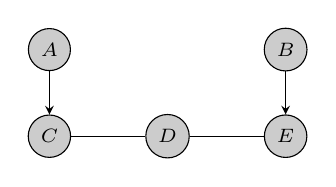
\begin{tikzpicture}
		\scriptsize
		\node[darkstyle] (a) at (-1.5,1.1) {$A$};
		\node[darkstyle] (c) at (-1.5,0) {$C$};
		\node[darkstyle] (d) at (0,0) {$D$};
		\node[darkstyle] (e) at (1.5,0) {$E$};
		\node[darkstyle] (b) at (1.5,1.1) {$B$};
		\draw[-stealth] (a)--(c);
		\draw[-stealth] (b)--(e);
		\draw (c)--(d);
		\draw (d)--(e);
		\end{tikzpicture}
	}
}

\begin{frame}{Chain Graphs}
\centering
\begin{figure}
\resizebox{0.6\textwidth}{!}{\upwardclosure}
\end{figure}
\begin{itemize}
	\item The \emph{upwardly closed subgraph} of $\boldsymbol{X}$, denoted
	$K^{+}[\boldsymbol{X}]$, is the induced subgraph over $\boldsymbol{Y}$,
	$K[\boldsymbol{Y}]$.
	\item Recursively expanding the boundary of $C$ in (a) yields the upward
	closure of $C$, which is $\{A,B,C,D,E\}$.
	\item The upwardly closed subgraph of $C$, $K^{+}[\{A,B,C,D,E\}]$, is
	shown in (b).
\end{itemize}
\end{frame}

\begin{frame}{Chain Graphs}
\begin{itemize}
	\item Let $K$ be a PDAG and $\boldsymbol{K}_{1}, \ldots,
	\boldsymbol{K}_{l}$ be its chain components. We define
	$\text{Pa}_{\boldsymbol{K}_{i}}$ to be the parents of the nodes in
	$\boldsymbol{K}_{i}$. The moralized graph of $K$ is an undirected graph
	$\mathcal{M}[K]$ produced by first connecting, using undirected edges,
	any pair of nodes $X,Y \in \text{Pa}_{\boldsymbol{K}_{i}} \,\forall i =
	1, \ldots, l$ and then converting all directed edges into undirected
	edges.
	\item The definition of the moralized graph here is the same as the the
	one discussed in the first talk, even for PDAGs.
\end{itemize}
\end{frame}

\begin{frame}{Chain Graphs}
\begin{itemize}
	\item Let $K$ be a PDAG, and $\boldsymbol{K}_{1}, \ldots,
	\boldsymbol{K}_{l}$ be its chain components. A chain graph distribution
	is defined via a set of factors $\phi_{i}(\boldsymbol{D}_{i})$ ($i = 1,
	\ldots, m$) such that each $\boldsymbol{D}_{i}$ is a complete subgraph
	in the moralized graph $\mathcal{M}[K^{+}[\boldsymbol{D}_{i}]]$.
	\item We associate each factor $\phi_{i}(\boldsymbol{D}_{i})$ with a
	single chain component $\boldsymbol{K}_{i}$ such that
	$\boldsymbol{D}_{i} \subseteq \boldsymbol{K}_{i} \cup
	\text{Pa}_{\boldsymbol{K}_{i}}$, and define $P(\boldsymbol{K}_{i})$ as a
	CRF with these factors, and with $\boldsymbol{Y}_{i} =
	\boldsymbol{K}_{i}$ and $\boldsymbol{X}_{i} =
	\text{Pa}_{\boldsymbol{K}_{i}}$.
\end{itemize}
\end{frame}

\begin{frame}{Chain Graphs}
\begin{itemize}
	\item We now define
	\[
		P(\mathcal{X}) = \prod_{i=1}^{l} P(\boldsymbol{K}_{i} \;|\;
		\text{Pa}_{\boldsymbol{K}_{i}}).
	\]
	\item We say that a distribution $P$ factorizes over $K$ if it can be
	represented as a chain graph distribution over $K$.
\end{itemize}
\end{frame}

\newcommand{\chaingraph}
{
	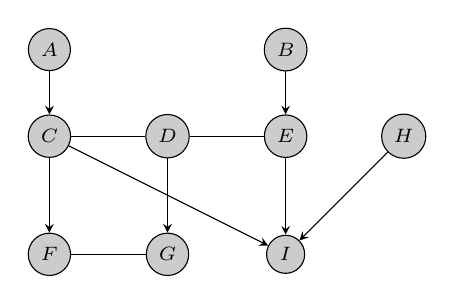
\begin{tikzpicture}
	\scriptsize
	\node[darkstyle] (a) at (-1.5,1.1) {$A$};
	\node[darkstyle] (c) at (-1.5,0) {$C$};
	\node[darkstyle] (d) at (0,0) {$D$};
	\node[darkstyle] (e) at (1.5,0) {$E$};
	\node[darkstyle] (b) at (1.5,1.1) {$B$};
	\node[darkstyle] (f) at (-1.5,-1.5) {$F$};
	\node[darkstyle] (g) at (0,-1.5) {$G$};
	\node[darkstyle] (i) at (1.5,-1.5) {$I$};
	\node[darkstyle] (h) at (3.0,0) {$H$};
	\draw[-stealth] (a)--(c);
	\draw[-stealth] (b)--(e);
	\draw[-stealth] (c)--(i);
	\draw[-stealth] (h)--(i);
	\draw[-stealth] (c)--(f);
	\draw[-stealth] (d)--(g);
	\draw[-stealth] (e)--(i);
	\draw (c)--(d);
	\draw (d)--(e);
	\draw (f)--(g);
	\end{tikzpicture}
}

\begin{frame}{Chain Graphs}
\centering
\resizebox{0.4\textwidth}{!}{\chaingraph}
\begin{itemize}
	\item In the chain graph shown above, we must have
	\[
		P(C,D,E \;|\; A,B) = \frac{1}{Z(A,B)}
		\phi_{1}(A,C)\phi_{2}(B,E)\phi_{3}(C,D)\phi_{4}(D,E).
	\]
	\item A similar factorization applies to $P(F,G \;|\; C,D)$.
\end{itemize}
\end{frame}

\begin{frame}{Independence}
\begin{itemize}
	\item Now that we know what a chain graph is, we will use our results
	from directed and undirected graphs to analyze how independence flows in
	a graph that incorporates both.
	\item Repeated for convenience: $\text{Boundary}_{X}$ is defined as the
	union of the parents of $X$ (all $Y$ such that $Y \rightarrow X$) and
	neighbors of $X$ (all $Y$ such that $Y \text{---} X$).
\end{itemize}
\end{frame}

\begin{frame}{Independence}
\begin{itemize}
	\item We define $\text{Descendants}_{X}$ to be the set of nodes that are
	reachable from $X$ via a directed path (one that involves at least one
	directed edge from $X$ to $Y$, but no directed edges from $Y$ to $X$).
	\item It follows that if $Y$ is a descendant of $X$, then $Y$ must be in
	a ``lower'' chain component.
\end{itemize}
\end{frame}

\begin{frame}{Independence}
\begin{itemize}
	\item For a PDAG $K$, we define the pairwise independencies associated
	with $K$ to be:
	\begin{gather*}
		I_{p}(K) = \{(X \perp Y \;|\; (\text{NonDescendants}_{X} -
		\{X,Y\})) :\\X,Y \,\textit{non-adjacent}, Y \in
		\text{NonDescendants}_{X}\}.
	\end{gather*}
	\item This generalizes the notion of pairwise independencies in directed
	graphs to undirected graphs: in an undirected graph,
	$\text{NonDescendants}_{X} = \mathcal{X}$.
\end{itemize}
\end{frame}

\begin{frame}{Independence}
\begin{itemize}
	\item For a PDAG $K$, we define the local independencies associated with
	$K$ to be:
	\begin{gather*}
		I_{\ell}(K) = \{(X \perp \text{NonDescendants}_{X} -
		\text{Boundary}_{X} \;|\;\\\text{Boundary}_{X} : X \in
		\mathcal{X})\}.
	\end{gather*}
	\item This generalization follows directly from the discussion of Markov
	blankets that was presented in the first talk.
	\item For directed graphs, $\text{NonDescendants}_{X}$ is precisely the
	set of nondescendants, whereas $\text{Boundary}_{X} = \pi(X)$.
	\item For undirected graphs, $\text{NonDescendants}_{X} = \mathcal{X}$,
	whereas $\text{Boundary}_{X} = \text{Nb}_{X}$.
\end{itemize}
\end{frame}

\newcommand{\chaingraphmoralization}
{
	\subfloat[][(a)]
	{%
		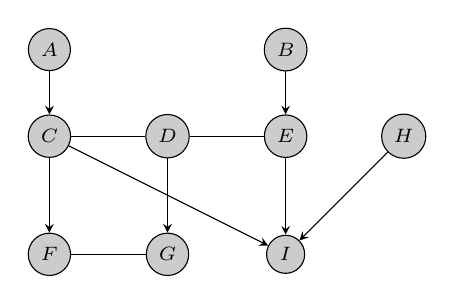
\begin{tikzpicture}
		\scriptsize
		\node[darkstyle] (a) at (-1.5,1.1) {$A$};
		\node[darkstyle] (c) at (-1.5,0) {$C$};
		\node[darkstyle] (d) at (0,0) {$D$};
		\node[darkstyle] (e) at (1.5,0) {$E$};
		\node[darkstyle] (b) at (1.5,1.1) {$B$};
		\node[darkstyle] (f) at (-1.5,-1.5) {$F$};
		\node[darkstyle] (g) at (0,-1.5) {$G$};
		\node[darkstyle] (i) at (1.5,-1.5) {$I$};
		\node[darkstyle] (h) at (3.0,0) {$H$};
		\draw[-stealth] (a)--(c);
		\draw[-stealth] (b)--(e);
		\draw[-stealth] (c)--(i);
		\draw[-stealth] (h)--(i);
		\draw[-stealth] (c)--(f);
		\draw[-stealth] (d)--(g);
		\draw[-stealth] (e)--(i);
		\draw (c)--(d);
		\draw (d)--(e);
		\draw (f)--(g);
		\end{tikzpicture}
	}%
	\hspace{0.7cm}
	\subfloat[][(b)]
	{%
		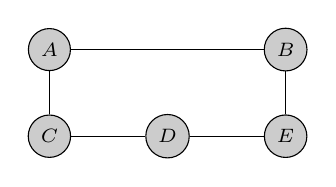
\begin{tikzpicture}
		\scriptsize
		\node[darkstyle] (a) at (-1.5,1.1) {$A$};
		\node[darkstyle] (c) at (-1.5,0) {$C$};
		\node[darkstyle] (d) at (0,0) {$D$};
		\node[darkstyle] (e) at (1.5,0) {$E$};
		\node[darkstyle] (b) at (1.5,1.1) {$B$};
		\draw (a)--(c);
		\draw (b)--(e);
		\draw (c)--(d);
		\draw (d)--(e);
		\draw (a)--(b);
		\end{tikzpicture}
	}
}

\begin{frame}{Independence}
\setlength{\topsep}{0pt}
\setlength{\partopsep}{0pt}
\centering
\begin{figure}
\resizebox{0.6\textwidth}{!}{\chaingraphmoralization}
\caption*{\scriptsize A chain graph $K$ and $\mathcal{M}[K^{+}[\{C,D,E\}]]$.}
\end{figure}
\begin{itemize}
	\item Let $\boldsymbol{X},\boldsymbol{Y}$ and $\boldsymbol{Z}$ be three
	disjoint sets, and let $\boldsymbol{U} = \boldsymbol{X} \cup
	\boldsymbol{Y} \cup \boldsymbol{Z}$. We say that $\boldsymbol{X}$ is
	c-separated from $\boldsymbol{Y}$ given $\boldsymbol{Z}$ if
	$\boldsymbol{X}$ is separated from $\boldsymbol{Y}$ given
	$\boldsymbol{Z}$ in the undirected graph
	$\mathcal{M}[K^{+}[\boldsymbol{X} \cup \boldsymbol{Y} \cup
	\boldsymbol{Z}]]$.
	\item In the figure above, $C$ is c-separated from $E$ given $D,A$,
	since $C$ is c-separated from $E$ given $D,A$ in the undirected graph.
	\item However, $C$ is not c-separated from $E$ given only $D$, since
	there a path from $C$ to $E$ in the undirected graph.
\end{itemize}
\end{frame}

\newcommand{\chaingraphmoralizationtwo}
{
	\subfloat[][(a)]
	{%
		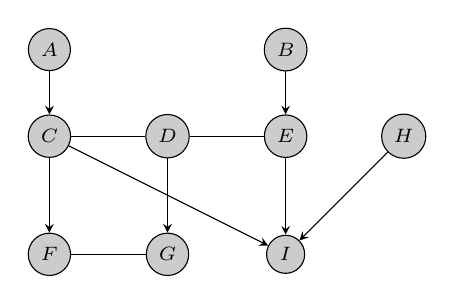
\begin{tikzpicture}
		\scriptsize
		\node[darkstyle] (a) at (-1.5,1.1) {$A$};
		\node[darkstyle] (c) at (-1.5,0) {$C$};
		\node[darkstyle] (d) at (0,0) {$D$};
		\node[darkstyle] (e) at (1.5,0) {$E$};
		\node[darkstyle] (b) at (1.5,1.1) {$B$};
		\node[darkstyle] (f) at (-1.5,-1.5) {$F$};
		\node[darkstyle] (g) at (0,-1.5) {$G$};
		\node[darkstyle] (i) at (1.5,-1.5) {$I$};
		\node[darkstyle] (h) at (3.0,0) {$H$};
		\draw[-stealth] (a)--(c);
		\draw[-stealth] (b)--(e);
		\draw[-stealth] (c)--(i);
		\draw[-stealth] (h)--(i);
		\draw[-stealth] (c)--(f);
		\draw[-stealth] (d)--(g);
		\draw[-stealth] (e)--(i);
		\draw (c)--(d);
		\draw (d)--(e);
		\draw (f)--(g);
		\end{tikzpicture}
	}%
	\hspace{0.7cm}
	\subfloat[][(b)]
	{%
		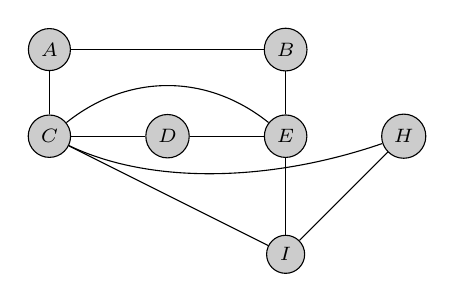
\begin{tikzpicture}
		\scriptsize
		\node[darkstyle] (a) at (-1.5,1.1) {$A$};
		\node[darkstyle] (c) at (-1.5,0) {$C$};
		\node[darkstyle] (d) at (0,0) {$D$};
		\node[darkstyle] (e) at (1.5,0) {$E$};
		\node[darkstyle] (b) at (1.5,1.1) {$B$};
		\node[darkstyle] (i) at (1.5,-1.5) {$I$};
		\node[darkstyle] (h) at (3.0,0) {$H$};
		\draw (a)--(c);
		\draw (b)--(e);
		\draw (c)--(i);
		\draw (h)--(i);
		\draw (e)--(i);
		\draw (c)--(d);
		\draw (d)--(e);
		\draw (a)--(b);
		\draw (c) .. controls (-0.5,0.8) and (0.5,0.8) .. (e);
		\draw (c) .. controls (-0.25,-0.6) and (1.25,-0.6) .. (h);
		\end{tikzpicture}
	}
}

\begin{frame}{Independence}
\setlength{\topsep}{0pt}
\setlength{\partopsep}{0pt}
\centering
\begin{figure}
\resizebox{0.6\textwidth}{!}{\chaingraphmoralizationtwo}
\caption*{\scriptsize A chain graph $K$ and $\mathcal{M}[K^{+}[\{C,D,E,I\}]]$.}
\end{figure}
\begin{itemize}
	\item The introduction of $I$ into the set of nodes in consideration
	results in a direct edge between $C$ and $E$ in the moralized graph, so
	we cannot render them independent by observing any of the other nodes.
\end{itemize}
\end{frame}

\begin{frame}{Independence}
\begin{itemize}
	\item Let $K$ be a PDAG. We define the global independencies associated
	with $K$ to be:
	\begin{gather*}
		I(K) = \{(\boldsymbol{X} \perp \boldsymbol{Y} \;|\;
		\boldsymbol{Z} : \boldsymbol{X},\boldsymbol{Y},\boldsymbol{Z}
		\subset \mathcal{X},\\
		\boldsymbol{X} \;\textit{is c-separated from}\; \boldsymbol{Y}
		\;\textit{given}\; \boldsymbol{Z})\}.
	\end{gather*}
	\item As in undirected graphs, if the distribution is positive:
	\begin{itemize}
		\item The three forms of independence and equivalent.
		\item $P$ factorizes over a PDAG $K$ if and only if $P \models
		I(K)$.
	\end{itemize}
\end{itemize}
\end{frame}

\begin{thebibliography}{11}
\bibitem{pgmbook}
Daphne Koller and Nir Friedman,
\emph{Probabilistic Graphical Models: Principles and Techniques},
MIT Press,
1st Edition,
2009.
\bibitem{pgmslides}
David Sontag, lecture slides on Probabilistic Graphical Models.
Accessible at \url{http://cs.nyu.edu/~dsontag/courses/pgm12/}.
\bibitem{nirslides}
Nir Friedman, lecture slides on the theory of Bayesian networks.
Accessible at \url{classes.soe.ucsc.edu/cmps290c/Spring04/paps/nir2.pdf}.
\end{thebibliography}

\end{document}
